\subsection{Effect of range of training data on map output} \label{subsec:comp_uncer}

To study how the range of training data affects map output accuracy and uncertainty, the difference between the map output and approximated measurement and the map output uncertainty for all available data points are plotted in Figure \ref{fig:rel_uncer}, and their uncertainty components are plotted in Figure \ref{fig:uncer_comp}.

\begin{figure}[h]
\begin{minipage}{15pc}
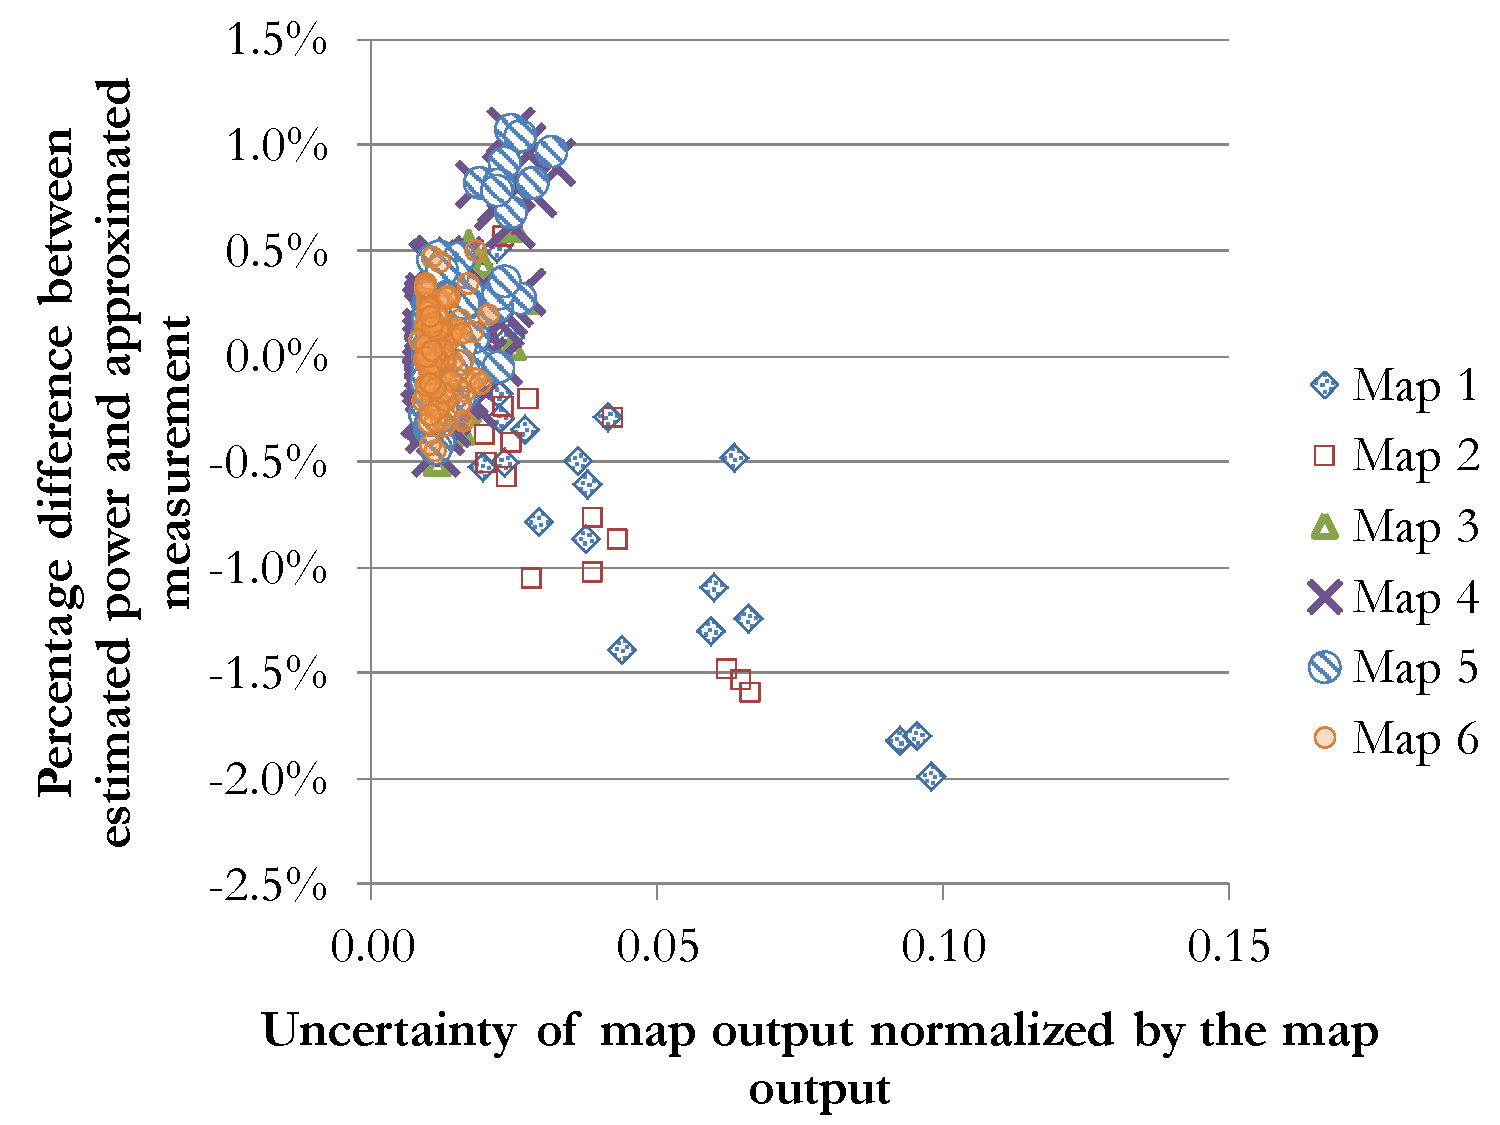
\includegraphics[width=15pc]{rel_diff_to_rel_uncer.pdf}
\caption{\label{fig:rel_uncer}Change of accuracy of maps with output uncertainty in different maps.}
\end{minipage}\hspace{2pc}%
\begin{minipage}{15pc}
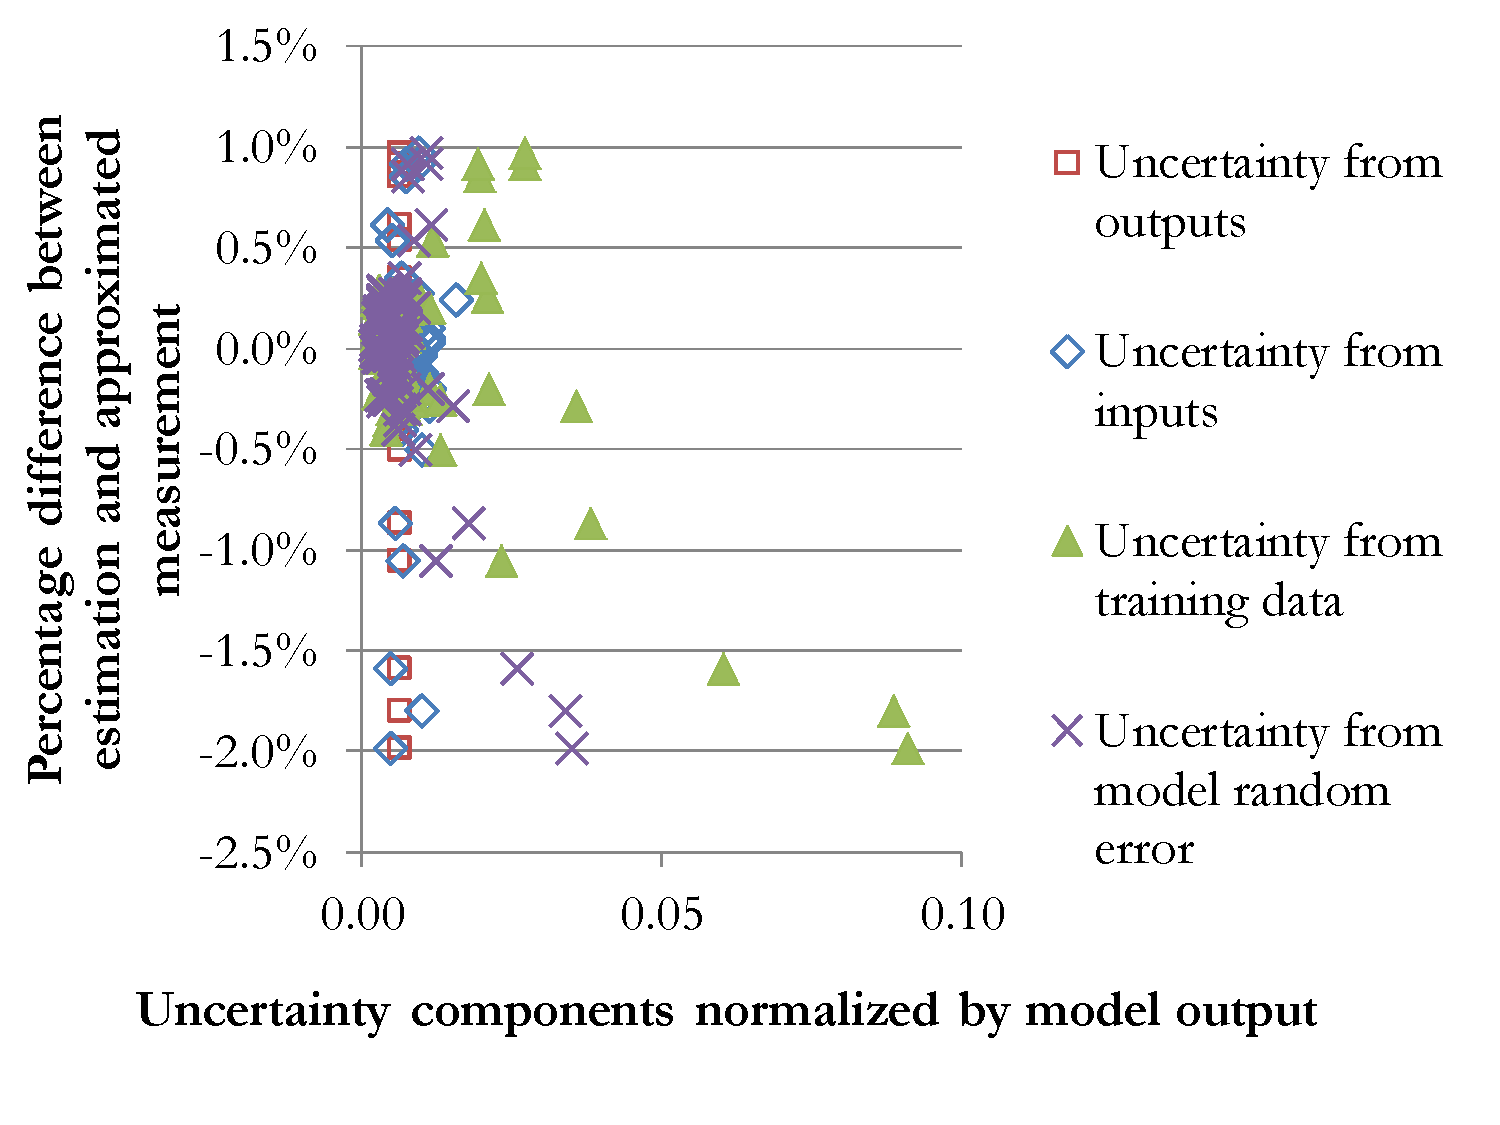
\includegraphics[width=15pc]{rel_diff_to_uncer_comp.pdf}
\caption{\label{fig:uncer_comp}Change of accuracy of maps with different uncertainty components.}
\end{minipage} 
\end{figure}

Figure \ref{fig:rel_uncer} shows that inaccurate map outputs are associated with higher uncertainty and the uncertainty calculation method is a good indicator of the accuracy of the map output. Figure \ref{fig:uncer_comp} shows that the high uncertainty of the inaccurate data points in Figure \ref{fig:rel_uncer} are results of high uncertainty from model random error and training data.

The increase of uncertainty from model random error with inaccuracy can be explained by the leverage term ${\vec x^T}{({\mathbf{X}}_{train}^T{{\mathbf{X}}_{train}})^{ - 1}}\vec x$ in Eqn. (\ref{eq:uncer_w_model}). When the inputs to the map become more different from the training data points o fthe map, the applicability and the accuracy of the map decrease. This is associated with an increase of leverage and the uncertainty from model random error. Hence the uncertainty of model random error increases as the applicability and the accuracy of the map decreases.

To explain the increase of uncertainty from training data with a decrease of map accuracy in Figure \ref{fig:uncer_comp}, the squared terms in Eqn. (\ref{eq:uncer_w_train}) are labeled as uncertainty from training data per measurement, and their values from two map outputs of Map 1 are plotted as histograms as shown in Figures \ref{fig:map_1_low_uncer} and \ref{fig:map_1_high_uncer}.

\begin{figure}[h]
\begin{minipage}{15pc}
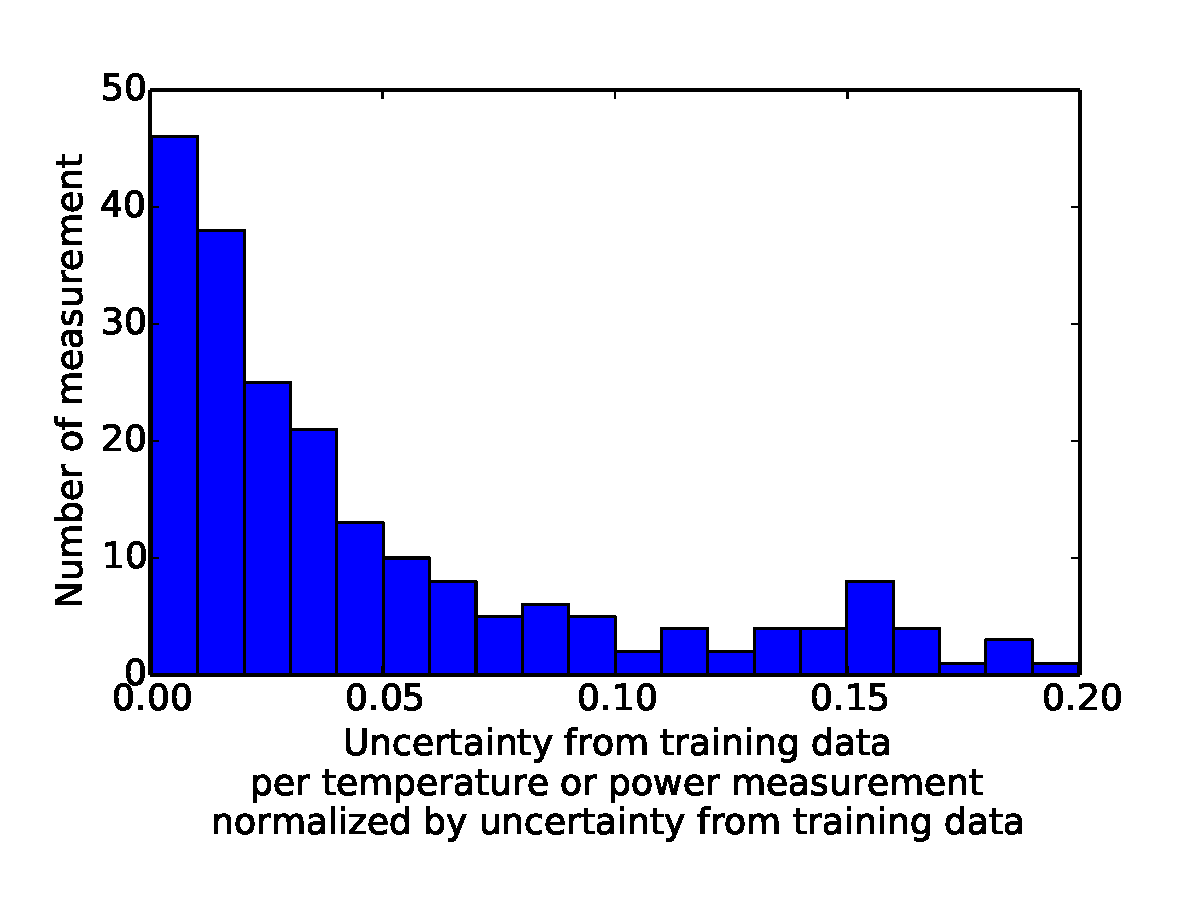
\includegraphics[width=15pc]{Map_1_low_uncer.pdf}
\caption{\label{fig:map_1_low_uncer}Histogram of uncertainty terms in Eqn. (\ref{eq:uncer_w_train}) for $T_{evap} = -1.1^\circ C$ and $T_{cond} = 60.0^\circ C$.}
\end{minipage}\hspace{2pc}%
\begin{minipage}{15pc}
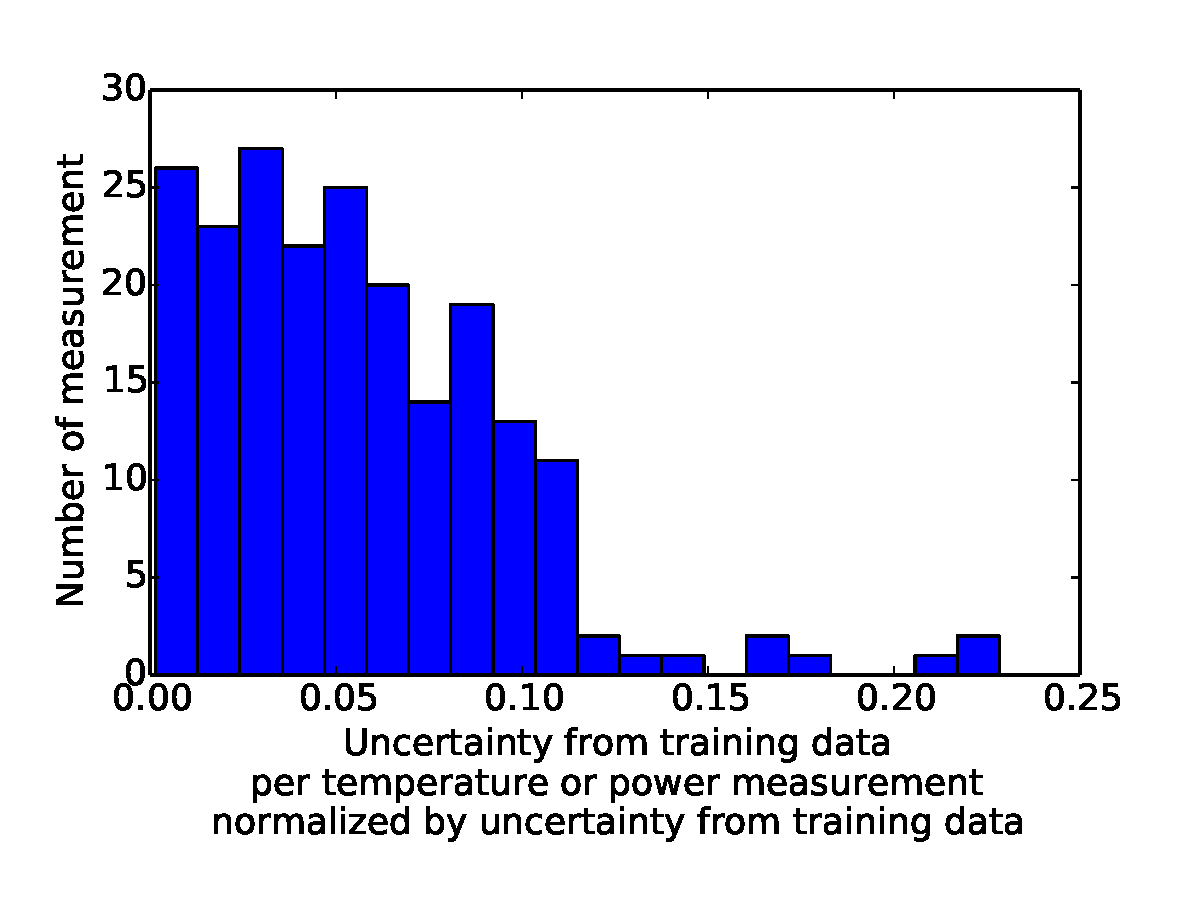
\includegraphics[width=15pc]{Map_1_high_uncer.pdf}
\caption{\label{fig:map_1_high_uncer}Histogram of uncertainty terms in Eqn. (\ref{eq:uncer_w_train}) for $T_{evap} = -28.9^\circ C$ and $T_{cond} = 26.7^\circ C$.}
\end{minipage} 
\end{figure}

Figure \ref{fig:map_1_low_uncer} shows a histogram that is more left-skewed than Figure \ref{fig:map_1_high_uncer}. This is because Figure \ref{fig:map_1_low_uncer} is obtained from a data point inside the training data range of Map 1 in Figure (FIGURE NUMBER TO BE ADDED FROM TEST CASE), and the map only needs information from a few data points around $T_{evap} = -1.1^\circ C$ and $T_{cond} = 60.0^\circ C$ to estimate its map output. Hence the estimation does not depend on most of the data points, and their training data uncertainties do not propagate to the map output as shown by Figure \ref{fig:map_1_low_uncer}. 

However, the map output at the condition in Figure \ref{fig:map_1_high_uncer} is conducted with the condition at the lower left handed corner in Figure (FIGURE NUMBER HERE), and is far away from most of the training data points of Map 1. To estimate the map output at this condition, the estimation is done by extrapolation and is significantly by multiple data points in the training data. If any of these significant training data points change, the estimation result at this condition will be changed significantly. Hence much more training data points propagate their uncertainty to the map output in Figure \ref{fig:map_1_high_uncer} than that in Figure \ref{fig:map_1_low_uncer}. This also explains that the uncertainty of training data is a significant component in the extrapolation uncertainty of the map output and it increases as the map applicability and accuracy decrease.
